\chapter{随机变量}

\begin{introduction}
    \item 离散与连续随机变量
    \item 一元与多元
    \item cdf, pmf, pdf
    \item 条件分布
    \item 独立随机变量
    \item 随机变量函数的分布
    \item 次序随机变量
\end{introduction}

在概率论中,主要关心$X$取值于数值集合$\mathcal{X}$中某个子集$B$的可能性,即希望得到$\P(\{\omega\in\Omega : X(\omega) \in B\})$。概率论不关心具体的样本点$\omega\in\Omega$,而关注其集合$\{\omega\in\Omega : X(\omega) \in B\}$,将其记为$X^{-1}(B)$。由于$\P$定义在$\mathscr{F}$上,故需$X^{-1}(B) \in \mathscr{F}$。

\begin{definition}[可测性]
    设所有值得关心的$B\subset \mathcal{X}$组成$\mathscr{F}_{\mathcal{X}}$,且$\forall B \in \mathscr{F}_{\mathcal{X}}$都满足$X^{-1}(B) \in \mathscr{F}$,则称$X$为$\mathscr{F}/\mathscr{F}_{\mathcal{X}}$\textbf{可测的}。当$\mathscr{F}_{\mathcal{X}}$不引起混淆时,简记为关于$\mathscr{F}$\textbf{可测},写作$X \in \mathscr{F}$。
\end{definition}

由于原像保持交、并、补等集合运算, 且$\mathscr{F}$是$\sigma$代数, 可将$\mathscr{F}_{\mathcal{X}}$扩张为合适的最小的$\sigma$代数, 即$\sigma(\mathscr{F}_{\mathcal{X}})$, 因此可测映射的定义不妨\underline{只考虑$\mathscr{F}_{\mathcal{X}}$是$\sigma$代数}的情况.

\begin{definition}[随机变量]
    为了表示因随机性而变动的量,称\underline{可测映射}(measurable mapping)
    \[ X : (\Omega,\mathscr{F},\P) \to (\mathcal{X},\mathscr{F}_{\mathcal{X}}), \quad \omega\in\Omega \mapsto X(\omega)\in\mathcal{X} \]
    为\textbf{随机元}(random element),也称\textbf{随机变量}(random variable)。其中$\mathscr{F}_{\mathcal{X}}$
\end{definition}

由于只考虑$\mathscr{F}_{\mathcal{X}}$是$\sigma$代数的情况,可将随机变量看作将原概率空间映射到新概率空间的方式。新样本空间为$\mathcal{X}$(一般由\underline{Borel点集}构成),新事件域为$\mathscr{F}_{\mathcal{X}}$,概率测度等于对应原像的。

\begin{remark}
    使用随机变量$X$时,有两个可能的含义:
    \begin{itemize}
        \item$X$的(随机)取值
        \item$X$的分布
    \end{itemize}
    例如若设$Y=-X, X \sim U(0,1)$,则两者对某样本点的取值是不同的,但两者的分布相同。
\end{remark}

\begin{definition}[随机向量]
    若随机变量$X_1(\omega), X_2(\omega),\cdots , X_n(\omega)$定义在\underline{同一概率空间}$(\Omega,\mathscr{F},\P)$上, 则称
    \[ X(\omega) = (X_1(\omega), X_2(\omega),\cdots , X_n(\omega)) \]
    构成一个n维\textbf{随机向量},亦称$n$维随机变量。
\end{definition}

\begin{definition}[离散与连续随机变量]
    若$\mathcal{X}$是(至多可数的)离散点集,$\mathscr{F}_{\mathcal{X}}$由$\mathcal{X}$的所有子集组成,则称$X$为\textbf{离散随机变量}(discrete random varible)。若$\mathcal{X} = \R^{n}$,$\mathscr{F}_{\mathcal{X}}$为$\{\prod_{i=1}^{n}(-\infty,x_{i}] : x_{1},\dots,x_{n}\in\R\}$生成的Borel代数(最小的$\sigma$代数),则称其为\textbf{连续随机变量}(continuous random varible)。
\end{definition}

\section{随机变量的分布}

\subsection{分布函数}

\begin{definition}[概率分布]
    称随机元$X$诱导的\underline{概率测度}
    \[ Q(\bullet)=\P\{X\in\bullet\},\ \bullet\in\mathscr{F}_{\mathcal{X}} \]
    为$X$的\textbf{概率分布}(distribution/law)。
\end{definition}
\begin{remark}
    对于随机变量,其取值是随机的,但其分布是固定的。
\end{remark}

\begin{definition}[单变量分布函数]
    若函数$F : \R \to [0,1] $满足以下性质,则称为单变量分布函数:
    \begin{description}
        \item[单调性] $F(x_1)\le F(x_2) , \quad \forall x_1<x_2$
        \item[有界性] $\lim_{n \to -\infty}F(x)=0, \quad \lim_{n \to \infty}F(x)=1$
        \item[右连续性] $\lim_{x \to x_0^+}F(x)=F(x_0)$
    \end{description}
\end{definition}

% \begin{property}
%   $F(x)$最多只有可数个间断点
% \end{property}

\begin{proposition}
    对每个分布$Q$都存在唯一一个分布函数$F_Q$使得$F_Q(x)=Q[(-\infty,x]], \quad \forall x \in \R$成立。
\end{proposition}
\begin{proof}
    \begin{align*}
        \because \      & \forall x_1>x_2 \in \mathbb{R},\ (-\infty,x_1]=(-\infty,x_2] \cup (x_2,x_1]     \\
        \therefore \    & \forall x_1>x_2 \in \mathbb{R},\ Q[(-\infty,x_1]]=Q[(-\infty,x_2]]+Q[(x_2,x_1]] \\
        \Rightarrow  \  & F_{Q}(x_1)=F_{Q}(x_2)+\P\{X\in(x_2,x_1]\}\ge F_{Q}(x_2)
    \end{align*}
    即$F_Q$满足单调性。

    由于$F_Q(x)=\P\{X\in(-\infty,x]\}$,所以$0\le F(x)\le 1$。由$F(x)$的单调性知,对任意整数$m$和$n$,有
    \[ \lim_{x \rightarrow-\infty} F(x)=\lim_{m \rightarrow-\infty} F(m),\ \lim_{x \rightarrow+\infty} F(x)=\lim_{n \rightarrow+\infty} F(n) \]
    又由概率的可列可加性得
    \begin{align*}
        1 & = P(-\infty<X<+\infty) = P\left(\bigcup_{i=-\infty}^{+\infty}\{i-1<X \le i\}\right)                                               \\
          & = \sum_{i=-\infty}^{+\infty} P(i-1<X \le i)=\lim_{n \rightarrow+\infty \atop m \rightarrow-\infty} \sum_{i =m}^{n} P(i-1<X \le i) \\
          & =\lim_{n \rightarrow+\infty} F(n)-\lim_{m \rightarrow-\infty} F(m)
    \end{align*}
    所以:
    \begin{gather}
        1 \le \lim_{n \rightarrow+\infty} F(n)=1+\lim_{m \rightarrow-\infty} F(m) \le 1 \\
        \lim_{n \rightarrow+\infty} F(n)=1 ,\ \lim_{m \rightarrow-\infty} F(m)=0
    \end{gather}
    即$F_Q$满足有界性。

    因为$F(x)$是单调有界非降函数,所以其任一点$x_0$的右极限$F(x_0+0)$必存在。右连续性的充要条件为:对任意单调下降的数列$x_1>x_2>\cdots>x_n>\cdots>x_0$,当$x_n \rightarrow x_0(n \rightarrow+\infty)$时,有$\lim _{n \rightarrow+\infty} F(x_n)=F(x_0)$。因为
    \begin{align*}
        F(x_1)-F(x_0) & =P(x_0 <X \le x_1)=P\left(\bigcup_{r=1}^{+\infty}\{x_{i+1}<X \le x_i\}\right)           \\
                      & =\sum_{i=1}^{+\infty} P(x_{i+1}<X \le x_i)=\sum_{i=1}^{+\infty}F(x_i)-F(x_{i+1})        \\
                      & =\lim _{n \rightarrow \infty}[F(x_1)-F(x_n)]=F(x_1)-\lim _{n \rightarrow \infty} F(x_n)
    \end{align*}
    即$F_Q$满足右连续性。
\end{proof}
\begin{note}
    由于$\{ x_1 \le x_0 \} \neq \bigcup_{r=1}^{+\infty}\{x_i < X \le x_{i+1}\}$,例$(-1,0]\neq \bigcup_{r=1}^{+\infty}(\frac{-1}{i},\frac{-1}{i+1}]=(-1,0)$。若将分布函数定义中右连续性改为左连续性,只需将命题改为$F_Q(x)=Q[(-\infty,x)], \quad \forall x \in \R$即可。
\end{note}

\begin{proposition}
    对每个分布函数$F$都存在唯一一个分布$Q_F$使得$Q_F[(-\infty,x]]=F(x), \quad \forall x \in \R$成立。
\end{proposition}
\begin{proof}
    参考\href{https://www.zhihu.com/question/23022012/answer/2520636971}{知乎}
\end{proof}

\begin{theorem}
    分布函数可以唯一决定概率分布,即:
    \[ Q_{F_Q}=Q, \quad F_{Q_F}=F \]
\end{theorem}
由此,概率分布与分布函数具有等同意义。所以可有以下定义:
\begin{definition}[随机变量的分布函数]
    设$X$是一个随机变量,其分布由分布函数:
    \[ F(x)=P(X \le x),\ \forall x \in \mathbb{R} \]
    唯一刻画,称为随机变量$X$的\textbf{(累积)分布函数}(cumulative distribution function, c.d.f.)。把随机变量$X$服从分布函数$F(x)$,简记作$X \thicksim F(x)$。
\end{definition}

\begin{figure}[h]
    \centering
    \subfloat[(累积)分布函数计算]{
        \begin{tikzpicture}
            \draw[->] (0,1)--(6,1);
            \draw[<-] (0,1.5)--(2,1.5);
            \draw[<-] (0,2)--(3,2);
            \draw[<-] (0,2.5)--(4,2.5);
            \draw[densely dotted] (2,1.5)--(2,1);
            \draw[densely dotted] (3,2)--(3,1);
            \draw[densely dotted] (4,2.5)--(4,1);
            \node (R) at(6,0.5) {$\mathbb{R}$};
            \node (x1) at(2,0.5) {x1};
            \node (x2) at(3,0.5) {x2};
            \node (x3) at(4,0.5) {x3};
            \fill (2,1.5) circle (2pt);
            \fill (3,2) circle (2pt);
            \fill (4,2.5) circle (2pt);
        \end{tikzpicture}
    }
    \subfloat[连续随机变量的分布函数]{
        \begin{tikzpicture}[>=stealth,xscale=1.8,yscale=2]
            \draw[->](-1.4,0)--(0,0)node[below left]{$O$}--(1.4,0)node[below]{$x$};
            \draw[->](0,-0.2)--(0,1.4)node[right]{$F(x)$};
            \draw[thick](-1,0)node[below]{$-1$}--(1,1)--(1.3,1);
            \draw[dashed,semithick](0,1)node[left]{$1$}--(1,1)--(1,0)node[below]{$1$};
        \end{tikzpicture}
    }

    \subfloat[离散随机变量的分布函数]{
        \begin{tikzpicture}[>=stealth]
            \draw[->](-2,0)--(0,0)node[below left]{$O$}--(3.5,0)node[below=1pt]{$x$};
            \draw[->](0,-0.5)--(0,2.5)node[left]{$F(x)$};
            \draw[thick](-2,0)--(-1,0)(-1,0.5)--(2,0.5)(2,1.5)--(3,1.5)(3,2)--(3.5,2);
            \fill(-1,0.5)circle(1pt);
            \fill(2,1.5)circle(1pt);
            \fill(3,2)circle(1pt);
            \filldraw[fill=white](-1,0)node[below]{$-1$}circle(1pt);\filldraw[fill=white](2,0.5)circle(1pt);
            \filldraw[fill=white](3,1.5)circle(1pt);
            \foreach \x in{1,2,3}\draw(\x,0.07)--(\x,0)node[below]{$\x$};
            \foreach \x in{1,1.5,2}\draw(0.07,\x)--(0,\x);
            \node[left]at(0,2){$1$};
        \end{tikzpicture}
    }
    \subfloat[既非离散、又非连续的分布函数]{
        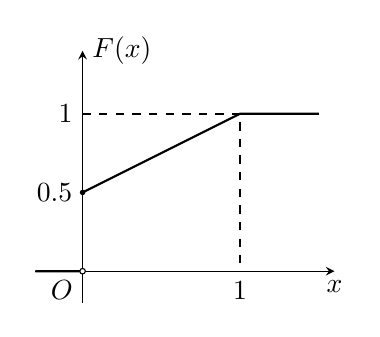
\begin{tikzpicture}[>=stealth,scale=2]
            \draw[->](-0.3,0)--(0,0)node[below left]{$O$}--(1.6,0)node[below]{$x$};
            \draw[->](0,-0.2)--(0,1.4)node[right]{$F(x)$};
            \draw[thick](0,0.5)node[left]{$0.5$}--(1,1)--(1.5,1)(-0.3,0)--(0,0);
            \filldraw[fill=white](0,0)circle(0.5pt);
            \fill(0,0.5)circle(0.5pt);
            \draw[semithick,dashed](0,1)node[left]{$1$}--(1,1)--(1,0)node[below]{$1$};
        \end{tikzpicture}
    }
    \caption{累积分布函数}
\end{figure}

% \begin{table}[h]
%     \centering
%     \begin{tabular}{|c|cc|}
%         \hline
%                                       & \multicolumn{1}{c|}{离散}                                 & 连续                        \\ \hline
%         \multirow{3}{*}{一元随机变量} & \multicolumn{1}{c|}{概率质量函数(pmf)}                    & 概率密度函数(pdf)           \\ \cline{2-3}
%                                       & \multicolumn{2}{c|}{累积分布函数(cdf)}                                                  \\ \cline{2-3}
%                                       & \multicolumn{2}{c|}{矩母函数/特征函数(mgf/chf)}                                         \\ \hline
%         \multirow{3}{*}{多元随机变量} & \multicolumn{1}{c|}{联合概率质量函数(joint pmf)}          & 联合概率密度函数(joint pdf) \\ \cline{2-3}
%                                       & \multicolumn{2}{c|}{联合累积分布函数(joint cdf)}                                        \\ \cline{2-3}
%                                       & \multicolumn{2}{c|}{联合矩母函数/特征函数(joint mgf/chf)}                               \\ \hline
%     \end{tabular}
% \end{table}

利用分布函数表示概率
\begin{align*}
     & P(a<X \le b) = F(b)-F(a),       \\
     & P(X=a) = F(a)-F(a-0),           \\
     & P(X \geq b) = 1-F(b-0),         \\
     & P(X>b) = 1-F(b),                \\
     & P(a<x<b) = F(b-0)-F(a),         \\
     & P(a \le X \le b) = F(b)-F(a-0), \\
     & P(a \le X<b) = F(b-0)-F(a-0).
\end{align*}

% \begin{proposition}
%     若$B_n$为$\R^n$上任一博雷尔点集,有
%     \[ \{ X(\omega) \in B_n \} \in \mathscr{F} \]
% \end{proposition}

\begin{definition}[随机向量的分布函数]
    若$n$元函数$F : \R^n \to [0,1] $满足:
    \[ F(x_1,x_2,\cdots,x_n)=\P \{ X_1(\omega)<x_1,X_2(\omega)<x_2,\cdots,X_n(\omega)<x_n \} \]
    则称其为随机向量$X(\omega)$的\textbf{联合分布函数}(joint cdf)。
\end{definition}

\begin{property}多元分布函数的一些性质:
    \begin{description}
        \item[单调性] 关于每个变元是单调不减函数;
        \item[有界性] \begin{align*}
                 & F(x_1,x_2, \cdots, -\infty, \cdots, x_n) & =0 \\
                 & F(+\infty,+\infty, \cdots, +\infty)      & =1
            \end{align*}
        \item[连续性] 关于每个变元右连续
            \[ F(x_1,x_2, \cdots, x_k+0, \cdots, x_n) =F(x_1,x_2, \cdots, x_k, \cdots, x_n),\ \forall x_i \in \mathbb{R} \]
        \item[非负性] 当$n=2$时,有
            \begin{equation}\label{equ:2dim_Prob}
                \P(a<X \le b, c<Y \le d)= F(b, d)-F(a, d)-F(b, c)+ F(a, c) \ge 0
            \end{equation}
    \end{description}
\end{property}
\begin{proof}
    单调性、有界性和右连续性的证明与单变量分布函数一样。对于非负性,只需证
    \[ P(a<X \le b, c<Y \le d)=F(b, d)-F(a, d)-F(b, c)+F(a, c) \]
    为此记 ( 见图~\ref{fig:3.1.2} )
    \[ A=\{X \le a\}, \quad B=\{ X \le b \}, \quad C=\{Y \le c\}, \quad D=\{Y \le d\} \]
    考虑到
    \[ \{ a<X \le b \}=B-A=B \cap \overline{A}, \quad\{c<Y \le d\}=D-C=D \cap \overline{C} \]
    且$A \subset B, C\subset D,$由此可得
    \begin{align*}
        0 & \le P(a<X \le b, c<Y \le d)                      \\
          & =P(B \cap \overline{A} \cap D \cap \overline{C}) \\
          & =P(B D-(A \cup C))                               \\
          & =P(B D)-P(A B D \cup B C D)                      \\
          & =P(B D)-P(A D \cup B C)                          \\
          & =P(B D)-P(A D)-P(B C)+P(A B C D)                 \\
          & =P(B D)-P(A D)-P(B C)+P(A C )                    \\
          & =P(B D)-P(A D)-P(B C)+P(A B C D)                 \\
          & =F(b, d)-F(a, d)-F(b, c)+F(a, c).
    \end{align*}
\end{proof}

\begin{figure}[htbp]
    \centering
    \begin{tikzpicture}[yscale=0.9]
        \draw [-Stealth] (-1,0) -- (0,0) node[below left]{$O$} -- (4,0) node[below] {$x$};
        \draw [-Stealth] (0,-1) -- (0,3) node[left] {$y$};
        \draw [thick] (1,1) -- (3,1) -- (3,2) -- (1,2) -- cycle;
        \draw [densely dashed] (1,1) -- (1,0) node[below] {$a$}
        (3,1) -- (3,0) node[below]{$b$} (1,1) -- (0,1) node[left] {$c$} (1,2) -- (0,2) node[left]{$d$};
    \end{tikzpicture}
    \caption{二维随机变量$(X,Y)$落在矩形中的情况}\label{fig:3.1.2}
\end{figure}

非负性式\ref{equ:2dim_Prob}是二维情况特有的,不能由前三条性质推出(反例见例\ref{ex:2dim_Prob_counter})。同理在$n=k$时,也可写出类似的等式,这是多元场合与一元场合的不同之处。

\begin{example}\label{ex:2dim_Prob_counter}
    设二元函数
    \[ G(x,y)=\begin{cases}
            0, & x+y < 0;  \\
            1, & x+y \ge 0 \\
        \end{cases}	\]
    $G(x,y)$具有非降性、有界性和右连续性,但在正方形区域$\{(x,y): -1\le x\le 1,-1\le y\le 1\}$的四个顶点上,右上三个顶点位于右上半闭平面,只有左下顶点$(-1,-1)$位于左下半开平面,故有:
    \[ G(1,1)-G(1,-1)-G(-1,1)+G(-1,-1)=1-1-1+0=-1<0 \]
    所以$G(x,y)$不满足式\ref{equ:2dim_Prob},故$G(x,y)$不能成为某二维随机变量的分布函数。
\end{example}

\begin{definition}[概率质量函数]
    若定义于至多可数点集$\X$的函数$p(x)$满足下述条件,则称其为\textbf{概率质量函数}(probability mass function, p.m.f.):
    \begin{gather*}
        p(x) \ge 0\\
        \sum_{x \in \X}p(x) = 1
    \end{gather*}
    当$p(\mathbf{x})$是多元函数时,则称其为\textbf{联合概率质量函数}(joint probability mass function, joint p.m.f.)
\end{definition}

设$X$为离散型随机变量,设$\mathscr{F}_{\mathcal{X}}$由$\mathcal{X}$的所有子集组成,此时$X$的分布由概率质量函数
\[ p_{X}(x) = \P\{X=x\} = \P(\{\omega\in\Omega:X(\omega)=x\}), \quad x\in\mathcal{X} \]
\underline{唯一}刻画。其与分布函数间有如下关系:
\begin{align*}
    F(x) & = \sum_{t\le x}P(X=t)=\sum_{t\le x}p(t) \\
    p(x) & = P(X=x)=F(x)-F(x_-)
\end{align*}
由于$p(x)$取值也为至多可列点集,故亦称其为$X$的\textbf{概率分布列}。

若$\mathbf{X}$为离散型随机向量,则只需将以上陈述改为多元情形即可。唯一不同的是由分布函数获取质量函数的方式,其应依照分布函数的非负性改为:
\[ p(x,y)=P(X=x,Y=y)=F(x, y)-F(x_-, y)-F(x, y_-)+ F(x_-, y_-) \]

\begin{definition}[概率密度函数]
    若定义于实数集$\X$的函数$f(x)$满足下述条件,则称其为\textbf{概率密度函数}(probability density function, p.d.f.):
    \begin{gather*}
        f(x) \ge 0 \\
        \int_{-\infty}^{\infty}f(x) \d x=1
    \end{gather*}
    当$f(\mathbf{x})$是多元函数时,则称其为\textbf{联合概率密度函数}(joint probability density function, joint p.d.f.)
\end{definition}

设$X$为连续型随机变量,且其分布函数$F(x)$可微,此时$X$的分布由
\[ f_{X}(x)\Delta x = P(x<X<x+\Delta x) \]
刻画。其与分布函数间的关系为:
\begin{align*}
    F(x) & = \int_{-\infty}^x f(t)\d t          \\
    f(x) & = \frac{\mathrm{d}F(x)}{\mathrm{d}x}
\end{align*}

若$\mathbf{X}$为连续型随机向量,则只需将以上陈述改为多元情形即可。唯一不同的也是由分布函数获取密度函数的方式,其应改为偏导:
\[ f(\mathbf{x}) := \frac{\partial^{n} F(\mathbf{x})}{\partial x_1 \cdots \partial x_n} \]

离散随机变量的分布函数$F(x)$总是右连续的阶梯函数,而连续随机变量的分布函数$F(x)$一定是整个数轴上的连续函数。因为对任意点$x$的增量$\Delta x$,相应分布函数的增量总有
\[ F(x+\Delta x)-F(x)=\int_{x}^{x+\Delta x} p(x) \dd  x \longrightarrow 0, \quad(\Delta x \rightarrow 0) \]

离散随机变量$X$在其可能取值的点$x_1, \cdots, x_n, \cdots$上的概率不为$0$。但即使对于$f(x)>0$的$x$,$P(X=x)=x\int_{x}^x f(t)dt=0$,即连续型随机变量在实轴上任意一点的概率测度为零。不可能事件的概率为$0$,但概率为$0$的事件不一定是不可能事件;类似地,必然事件的概率为$1$,但概率为$1$的事件不一定是必然事件。概率密度函数$f(x)$代表的是在此位置上单位长度的概率,可能是一个很大的值。

由于连续随机变量$X$仅取一点的概率恒为$0$,从而在事件$\{ a \le X \le b \}$中减去$X=a$或减去$X=b$,不影响其概率,即
\[ P(a \le x \le b)=P(a<X \le b)=P(a \le X<b)=P(a<X<b) \]
由于在若干点上改变密度函数$f(x)$的值并不影响其积分的值,从而不影响其分布函数$F(x)$的值,即连续分布的密度函数不唯一。

\subsection{边际分布与条件分布}

\begin{definition}[边际分布]
    对于多维随机变量$X$,将其中一个分量的分布称为$X_i$的\textbf{边际分布}。对于分量$X_i$,其\textbf{边际分布函数}(marginal cdf)为:
    \[ F_{X_i}(x_i) = \P\{ X_i \le x_i \} = F(\infty,\cdots , x_i ,\cdots ,\infty)\]
\end{definition}

\begin{definition}[边际质量函数与边际密度函数]
    对于多维离散(连续)随机变量$X$,将其中一个分量$X_i$对应的质量函数(密度函数)称为$X_i$的\textbf{边际质量函数(边际密度函数)}。此时,边际质量函数(边际密度函数)即可通过边际分布函数获得:
    \[ p_{X_i}(x_i)=F_{X_i}(x_i)-F_{X_i}(x_{i-}), \quad f_{X_i}(x_i)=\frac{\d F_{X_i}}{\d x_i}(x_i) \]
    也可通过质量函数(密度函数)获得:
    \[ p_{X_i}(x_i)=\sum_{\mathbf{x}\in \mathcal{X}_i(x_i)}p(\mathbf{x}), \quad f_{X_i}(x_i)=\int_{\mathbf{x}\in \mathcal{X}_i(x_i)}f(\mathbf{x})\d \mathbf{x} \]
    其中$\mathcal{X}_i(a)=\{ \mathbf{x} \in \mathcal{X} : x_i=a \}$。
\end{definition}

\begin{definition}[独立随机变量]
    若随机向量$\mathbf{X}(\omega) = (X_1(\omega), X_2(\omega),\cdots , X_n(\omega))$联合分布函数可分解成各分量边缘分布函数的乘积,即:
    \[ F(x_1,x_2,\cdots ,x_n) = F_{X_1}(x_1)F_{X_2}(x_2)\cdots F_{X_n}(x_n) , \quad \forall x_1,x_2,\cdots ,x_n \in \R \]
    则称随机向量$\mathbf{X}$各分量相互\textbf{独立}
\end{definition}
\begin{remark}
    对于一般的多元随机变量,其各分量边缘分布不足以描述联合分布的情况;但若其各分量独立,则可以。
\end{remark}

\begin{theorem}\label{thm:indep_cmf}
    对于连续情况:
    \begin{align*}
                        & F(x_1,x_2,\cdots ,x_n) = F_{X_1}(x_1)F_{X_2}(x_2)\cdots F_{X_n}(x_n) \\
        \Leftrightarrow & f(x_1,x_2,\cdots ,x_n) = f_{X_1}(x_1)f_{X_2}(x_2)\cdots f_{X_n}(x_n)
    \end{align*}
    对于离散情况:
    \begin{align*}
                        & F(x_1,x_2,\cdots ,x_n) = F_{X_1}(x_1)F_{X_2}(x_2)\cdots F_{X_n}(x_n) \\
        \Leftrightarrow & p(x_1,x_2,\cdots ,x_n) = p_{X_1}(x_1)p_{X_2}(x_2)\cdots p_{X_n}(x_n)
    \end{align*}
\end{theorem}
\begin{remark}
    分解函数时应注意其自变量的取值范围是否粘连。若相互粘连,则必不能分解。
\end{remark}

设二维连续随机变量$(X,Y)$的联合密度函数为$f(x,y)$,边际密度函数为$p_X(x),p_Y(y)$。在离散随机变量场合,其条件分布函数为$P(X \le x|Y=y)$。但由于连续随机变量取某个值的概率为零,即$P(Y=y)=0$,所以无法用条件概率直接计算$P(X \le x|Y=y)$。一个很自然的想法是:将$P(X \le x|Y=y)$看成$h \to 0$时,$P(X \le x|y \le Y \le y+h)$的极限(在离散情况下,此式也成立),即:
\begin{align*}
    P(X \le x|Y=y) & = \lim_{h \to 0} P(X \le x|y \le Y \le y+h)                                                                                           \\
                   & = \lim_{h \to 0} \frac{P(X \le x, y \le Y \le y+h)}{P(y \le Y \le y+h)}                                                               \\
                   & =\lim_{h \to 0} \frac{\int_{-\infty}^{x} \int_y^{y+h} f(u,v) \d v \d u}{\int_y^{y+h} f_Y(v) \d v}                                     \\
                   & =\lim_{h \to 0} \frac{\int_{-\infty}^{x} \left\{ \frac1{h} \int_y^{y+h} f(u, v) \d v \right\} \d u}{\frac1{h} \int_y^{y+h} f_Y(v) dv}
\end{align*}
当$f_Y(y),p(x,y)$在$y$处连续时,由积分中值定理可得:
\begin{align*}
     & \lim_{h \to 0} \frac1{h} \int_y^{y+h} f_Y(v) dv=f_Y(y)    \\
     & \lim_{h \to 0} \frac{1}{h} \int_y^{y+h} f(u, v) dv=f(u,y)
\end{align*}
所以
\[ P(X \le x |Y=y)=\int_{-\infty}^{x} \frac{p(u, y)}{p_Y(y)} \d u \]
至此,可以定义随机变量的条件分布如下:
\begin{definition}[条件分布]\label{def:cond_dist}
    对一切使$f_Y(y)>0$的$y$,给定$Y=y$条件下$X$的\textbf{条件分布函数}和\textbf{条件密度函数}分别为
    \begin{align*}
         & F(x | y)=\int_{-\infty}^{x} \frac{f(u, y)}{f_Y(y)} \d u, \\
         & f(x | y)=\frac{f(x, y)}{f_Y(y)}.
    \end{align*}
\end{definition}

\begin{remark}
    对于每一个\underline{固定的$x$},$p_{Y|X}(y|x)$是一个关于$y$的概率质量函数;$f_{Y|X}(y|x)$是一个关于$y$的概率密度函数
\end{remark}

\begin{example}\label{exam:3.5.2}
    设随机变量 $X$ 与 $Y$ 相互独立, 且 $X\sim P(\lambda_1),Y\sim P(\lambda_2)$. 在已知 $X+Y=n$ 的条件下, 求 $X$ 的条件分布.
\end{example}
\begin{solution}
    因为独立泊松变量的和仍为泊松变量, 即 $X+Y\sim P(\lambda_1+\lambda_2)$, 所以
    \begin{align*}
        P(X=k | X+Y=n) & =\frac{P(X=k, X+Y=n)}{P(X+Y=n)}                                                                   \\
                       & =\frac{P(X=k) P(Y=n-k)}{P(X+Y=n)}                                                                 \\
                       & =\frac{\frac{\lambda_1^k}{k!}\ee^{-\lambda_1}\cdot\frac{\lambda_2^{n-k}}{(n-k)!}\ee^{-\lambda_2}}
        {\frac{(\lambda_1+\lambda_2)^n}{n!}\ee^{-(\lambda_1+\lambda_2)}}                                                   \\
                       & =\frac{n!}{k!(n-k)!}\frac{\lambda_1^k\lambda_2^{n-k}}{(\lambda_1+\lambda_2)^n}                    \\
                       & =\binom{n}{k}\left(\frac{\lambda_1}{\lambda_1+\lambda_2}\right)^k
        \left(\frac{\lambda_2}{\lambda_1+\lambda_2}\right)^{n-k},\quad k=0,1,\dots,n.
    \end{align*}
    即在 $X+Y=n$ 的条件下, $X$ 服从二项分布 $b(n,p)$, 其中 $p=\lambda_1/(\lambda_1+\lambda_2)$.
\end{solution}

\begin{example}\label{exam:3.5.4}
    设$(X,Y)$服从二维正态分布$N(u_1,u_2,\sigma_1^2,\sigma_2^2,\rho)$,由边际分布知$X \sim N(\mu_1,\sigma_1^2), Y \sim N(\mu_2,\sigma_2^2)$服从正态分布。分别求$X,Y$条件分布。
\end{example}
\begin{solution}
    \begin{align*}
        f(x \mid y) & =\frac{f(x, y)}{f_Y(y)}                                                                                                                                                                                                                                                                                            \\
                    & =\frac{\frac1{2 \pi \sigma_1 \sigma_2 \sqrt{1-\rho^2}} \exp \left\{-\frac1{2(1-\rho^2)}\left[\frac{(x-\mu_1)^2}{\sigma_1^2}-2 \rho \frac{(x-\mu_1)(y-\mu_2)}{\sigma_1 \sigma_2}+\frac{(y-\mu_2)^2}{\sigma_2^2}\right]\right\}}{\frac1{\sqrt{2 \pi} \sigma_2}\exp \left\{-\frac{(y-\mu_2)^2}{2 \sigma_2^2}\right\}} \\
                    & =\frac1{\sqrt{2 \pi} \sigma_1 \sqrt{1-\rho^2}} \exp \left\{-\frac1{2 \sigma_1^2(1-\rho^2)}\left[x-\left(\mu_1+\rho \frac{\sigma_1}{\sigma_2}(y-\mu_2)\right)\right]^2\right\}
    \end{align*}
    这正是正态密度函数,其均值$\mu_3$和方差$\sigma_3^2$分别为
    \[ \mu_{3}=\mu_{1}+\rho \frac{\sigma_{1}}{\sigma_{2}}\left(y-\mu_{2}\right),\quad \sigma_{3}^{2}=\sigma_{1}^{2}\left(1-\rho^{2}\right) \]
    类似可得, 在给定$X=x$的条件下,$Y$的条件分布仍为正态分布$N(\mu_4,\sigma_4^2)$, 其均值和方差分别为
    \[ \mu_{4}=\mu_{2}+\rho \frac{\sigma_{2}}{\sigma_{1}}\left(x-\mu_{1}\right),\quad \sigma_{4}^{2}=\sigma_{2}^{2}\left(1-\rho^{2}\right) \]
\end{solution}
由此也可以看出:二维正态分布的边际分布和条件分布都是一维正态分布,这是正态分布的一个重要性质.

\textbf{与概率三定理的对应}:
\begin{description}
    \item[乘法法则] $p_{XY}(x,y)=p_{Y|X}(y|x)p_{X}(x), \quad f_{XY}(x,y)=f_{Y|X}(y|x)f_{X}(x)$
    \item[全概率公式] $p_Y(y)=\sum_{x}p_{Y|X}(y|x)p_{X}(x), \quad f_Y(y)=\int^{+\infty}_{-\infty}f_{Y|X}(y|x)f_{X}(x)dx$
    \item[Bayes原理] $p_{X|Y}(x|y)=\frac{p_{Y|X}(y|x)p_{X}(x)}{\sum_{x}p_{Y|X}(y|x)p_{X}(x)}, \quad f_{X|Y}(x|y)=\frac{f_{Y|X}(y|x)f_{X}(x)}{\int^{+\infty}_{-\infty}f_{Y|X}(y|x)f_{X}(x)dx}$
\end{description}

\begin{example}
    设在一段时间内进入某一商店的顾客人数$X \sim P(\lambda)$,每个顾客购买某种物品的概率为$p$,并且各个顾客是否购买该种物品相互独立,求进人商店的顾客购买这种物品的人数$Y$的分布列。
\end{example}
\begin{solution}
    由题意知
    \[ P\{X=m\}=\frac{\lambda^m}{m!} \ee^{-\lambda}, \quad m=0,1,2, \dots \]
    在进人商店的人数$X=m$的条件下,购买某种物品的人数$Y$的条件分布为二项分布$b(m,p)$,即
    \[ P\{ Y=k | X=m \}=\binom{m}{k}p^k(1-p)^{m-k}, \quad k=0,1,2, \dots, m \]
    由全概率公式有
    \begin{align*}
        P\{Y=k\} & =\sum_{m=k}^{+\infty} P\{X=m\}P\{Y=k | X=m\}                                                       \\
                 & =\sum_{m=k}^{+\infty} \frac{\lambda^m}{m!} \ee^{-\lambda} \cdot \frac{m!}{k!(m-k)!} p^k(1-p)^{m-k} \\
                 & =\ee^{-\lambda} \sum_{m=k}^{+\infty} \frac{\lambda^m}{k!(m-k)!} p^k(1-p)^{m-k}                     \\
                 & =\ee^{-\lambda} \frac{(\lambda p)^k}{k!} \sum_{m=k}^{+\infty} \frac{[(1-p) \lambda]^{m-k}}{(m-k)!} \\
                 & =\frac{(\lambda p)^k}{k!} \ee^{-\lambda p}, \quad k=0,1,2, \dots.
    \end{align*}
\end{solution}
即$Y$服从参数为$\lambda p$的泊松分布.

这个例子告诉我们: 在直接寻求$Y$的分布有困难时, 有时借助条件分布可把困难克服了.

\begin{example}\label{exam:3.5.6}
    设$X\sim N(\mu,\sigma_1^2)$,在$X=x$的条件下$Y|X=x\sim N(x,\sigma_2^2)$。试求$Y$的(无条件)密度函数$p_Y(y)$。
\end{example}
\begin{solution}
    由题意知
    \begin{align*}
        p_{X}(x) & =\frac{1}{\sqrt{2 \pi} \sigma_{1}} \exp \left\{-\frac{(x-\mu)^{2}}{2 \sigma_{1}^{2}}\right\}, \\
        p(y | x) & =\frac{1}{\sqrt{2 \pi} \sigma_{2}} \exp \left\{-\frac{(y-x)^{2}}{2 \sigma_{2}^{2}}\right\}.
    \end{align*}
    所以
    \begin{align*}
        p_{Y}(y) & =\int_{-\infty}^{+\infty} p_{X}(x) p(y | x) \dd x                                               \\
                 & =\frac{1}{2 \pi \sigma_{1} \sigma_{2}} \int_{-\infty}^{+\infty}\exp \left\{-\frac{(x-\mu)^{2} }
        {2 \sigma_{1}^{2}}-\frac{(y-x)^{2}}{2 \sigma_{2}^{2}}\right\} \dd x                                        \\
                 & =\frac{1}{2 \pi \sigma_{1} \sigma_{2}} \int_{-\infty}^{+\infty}
        \exp \left\{-\frac{1}{2}\left[\left(\frac{1}{\sigma_{1}^{2}}+\frac{1}{\sigma_{2}^{2}}\right) x^{2}-2\left(\frac{y}{\sigma_{2}^{2}}+\frac{\mu}{\sigma_{1}^{2}}\right) x+\frac{y^{2}}{\sigma_{2}^{2}}\right]\right\} \dd x .
    \end{align*}
    记$c=\frac{\sigma_{1}^{2} \sigma_{2}^{2}}{\sigma_{1}^{2}+\sigma_{2}^{2}}$, 则上式化成
    \begin{align*}
        p_{Y}(y) & =\frac{1}{2 \pi \sigma_{1} \sigma_{2}} \int_{-\infty}^{+\infty} \exp \left\{-\frac{1}{2} c^{-1}\left[x-c\left(\frac{\mu}{\sigma_{1}^{2}}+\frac{y}{\sigma_{2}^{2}}\right)\right]^{2}-\frac{1}{2} \frac{(y-\mu)^{2}}{\sigma_{1}^{2}+\sigma_{2}^{2}}\right\} \dd x \\
                 & =\frac{1}{2 \pi \sigma_{1} \sigma_{2}} \sqrt{2 \pi c} \exp \left\{-\frac{(y-\mu)^{2}}{2\left(\sigma_{1}^{2}+\sigma_{2}^{2}\right)}\right\}                                                                                                                      \\
                 & =\frac{1}{\sqrt{2 \pi} \sqrt{\sigma_{1}^{2}+\sigma_{2}^{2}}} \exp \left\{-\frac{(y-\mu)^{2}}{2\left(\sigma_{1}^{2}+\sigma_{2}^{2}\right)}\right\} .
    \end{align*}
    这表明$Y$仍服从正态分布$N(\mu,\sigma_1^2+\sigma_2^2)$.
\end{solution}

\section{随机变量的函数}

在统计学中,常需要转化原始数据以获取其中信息,由此引出了研究随机变量的函数的需要。

\begin{theorem}[随机变量的函数的分布]
    设$Y=g(X)$是随机向量$X=(X_1,X_2,\cdots ,X_n)$的函数,则$Y$的分布由$X$的分布通过下式决定:
    \[ \P\{Y \in B\} = \P\{X \in A\}, \quad A=\{ \omega |g(X(\omega))\in B\} \]
\end{theorem}

此法是其他方法的基础,但使用不便,常用于离散随机变量。

\begin{example}[离散卷积公式]\label{exp:sum_of_pmf}
    已知离散随机变量$X,Y$的联合概率质量函数为$p(x,y)$, 求$Z=X+Y$的分布
\end{example}
\begin{solution}
    \[ p_Z=P(Z=z)=P(X+Y=z)=\sum_{x=-\infty}^{\infty}p(x, z-x) \]
    若$X,Y$独立,则$p_Z(z)=\sum_{-\infty}^{\infty}p_X(x)p_Y(z-x)dx$,为$p_X$与$p_Y$的卷积。
\end{solution}

\begin{theorem}[]
    若随机变量$X,Y$独立,则其变换$Z=g(X), W=h(Y)$也独立。

    泛化情况:若随机向量$\{X\}_n$各分量独立,则其变换$\{Y\}_n=g(\{X\}_n)$各分量也独立。
\end{theorem}
\begin{proof}
    %TODO: 待补
\end{proof}

\subsection{分布函数法}

通过下式获取随机变量的函数的分布函数:
\[ F_Y(y)=\begin{cases}
        \int_{A_y}f_X(\mathbf{x})\d\mathbf{x} \\
        \sum_{\mathbf{x} \in A_y}p_X(\mathbf{x})
    \end{cases}   \quad A_y=\{ \mathbf{x}|g(\mathbf{x}) \le y \} \]

对每一个变换分别运用上式则可得到向量函数的分布.

\begin{example}
    已知随机变量$X$的概率密度函数$f_X(x)$与分布函数$F_X(x)$, 求$Y=X^2$的分布
\end{example}
\begin{solution}
    易知,若$y<0$,则$F_Y(y)=0,f_Y(y)=0$;若$y\ge 0$,则:
    \begin{align*}
        F_Y(y)=P(Y\le y)           & =P(-\sqrt{y}<X\le \sqrt{y})+P(X=\sqrt{y})                             \\
                                   & =F_X(\sqrt{y})-F_X(-\sqrt{y})+0                                       \\
        f_Y(y) =\frac{d}{dy}F_Y(y) & =\frac{d}{dy}F_X(\sqrt{y}) -\frac{d}{dy}F_X(\sqrt{y})                 \\
                                   & =f_X(\sqrt{y})\frac{1}{2\sqrt{y}} -f_X(-\sqrt{y})\frac{-1}{2\sqrt{y}} \\
                                   & =\frac1{2\sqrt{y}}[f_X(\sqrt{y})+f_X(-\sqrt{y})]
    \end{align*}
\end{solution}

\begin{example}[连续变量之和]\label{exp:sum_of_pdf}
    已知随机变量$X,Y$的联合概率密度函数$f(x,y)$, 求$Z=X+Y$的分布
\end{example}
\begin{solution}
    \begin{align*}
        F_Z(z) & =P(Z\le z)=P(X+Y\le z)                                                    \\
               & =\iint_{x+y\le z}f(x,y)\d x \d y                                          \\
               & =\int_{-\infty}^{+\infty}\int_{-\infty}^{z-x}f(x,y) \d y \d x             \\
               & =\int_{-\infty}^{z}\int_{-\infty}^{\infty}f(x,v-x)\d x \d v, \quad y= v-x \\
        f_Z(z) & =\frac{d}{dz}F_Z(z)=\int_{-\infty}^{\infty}f(x,z-x)\d x
    \end{align*}
    若$X,Y$独立,则$f_Z(z)=\int_{-\infty}^{\infty}f_X(x)f_Y(z-x)dx$,为$f_X$与$f_Y$的卷积,记为$F_X(x|\theta_X)*F_Y(y|\theta_Y)$,与例\ref{exp:sum_of_pmf}类似
\end{solution}

\begin{example}[连续变量之商]\label{ex:quotient_of_variable}
    已知随机变量$X,Y$的联合概率密度函数$f(x,y)$, 求$Z=\frac{Y}{X}$的分布
\end{example}
\begin{solution}
    \[ Q_{z}=\{(x, y): y / x \le z\}=\{(x, y): x<0, y \geq z x\} \cup\{(x, y): x>0, y \le z x\} \]
    \begin{align*}
        F_{Z}(z) & =\iint_{Q_{z}} f(x, y) d x d y=\int_{-\infty}^{0} \int_{x z}^{\infty}+\int_{0}^{\infty} \int_{-\infty}^{x z} f(x, y) d y d x \\
                 & =\int_{-\infty}^{0} \int_{z}^{-\infty}+\int_{0}^{\infty} \int_{-\infty}^{z} x f(x, x v) d v d x \quad(\text{set} y=x v)      \\
                 & =\int_{-\infty}^{0} \int_{-\infty}^{z}(-x) f(x, x v) d v d x+\int_{0}^{\infty} \int_{-\infty}^{z} x f(x, xv) dvdx            \\
                 & =\int_{-\infty}^{z} \int_{-\infty}^{\infty}|x| f(x, xv) dxdv                                                                 \\
        f_Z(z)   & =\frac{d}{dz}F_Z(z)=\int_{-\infty}^{\infty}|x|f(x,xz)dx
    \end{align*}
\end{solution}

\subsection{Copula}\label{subsec:Copula}

\begin{definition}
    设\underline{连续型}实值随机变量$X$有分布函数$F$, 易见$F$在$\overline{\R}=[-\infty,+\infty] $上从$0$递增到$1$. 定义相应的\textbf{分位数函数}(quantile function)为
    \[ F^{-1}(p) := \inf\{x\in\R:F(x)\ge p\}, \quad p \in [0,1]. \]
\end{definition}
\begin{remark}
    当$F$严格递增时, 这与一般的反函数定义相同.
\end{remark}

\begin{theorem}\label{thm:pseudo_random_generation}
    设\underline{连续型}实值随机变量$X$分布函数为$F$,则$F(X) \sim \U(0,1)$。若设$U \sim \U([0,1])$,则$F^{-1}(U) \overset{d}{=} X$, 其中$\overset{d}{=}$表示分布相同(equal in distribution)。
\end{theorem}
\begin{proof}
    \[ \P\{F(X)\le p\} = \P\{X\le F^{-1}(p)\} = F(F^{-1}(p)) =p, \quad \forall p \in [0,1]. \]
\end{proof}

\begin{remark}
    设随机变量$Y=h(U)$,然而$h^{-1}(y)$未必等于其分布函数$F_Y(y)$,只有当$h^{-1}(y)$满足分布函数条件时两者才相等。
\end{remark}

% \begin{theorem}[Sklar定理]
%     考虑多个\underline{连续型}实值随机变量$X_{1},\dots,X_{k}$, 记$X_{i}$的分布函数为$F_{i}$. 我们称$(F_{1}(X_{1}),\dots,F_{k}(X_{k}))$的分布函数$C : [0,1]^k \to [0,1] $为相应的\textbf{Copula}, 适合
%     \[ C(F_{1}(x_{1}),\dots,F_{k}(x_{k})) = \P\{X_{1}\le x_{1},\dots,X_{k}\le x_{k}\}, \quad \forall x_{1},\dots,x_{k} \]
%     这个结果称为\textbf{Sklar定理}
% \end{theorem}
% 这个结果, 在金融统计中有颇多应用. 稍作诠释的话, Copula提取了变量间的\emph{相关性}, 通过粘合\emph{边际}能够恰好地表示\emph{总体}.人们可以构造各种各样的Copula, 对真实世界进行建模.

\subsection{概率密度函数法}

\begin{theorem}[单变量函数的概率函数变换]
    设连续随机变量$X$的概率密度函数为$f_X(x)$,若随机变量$Y=g(X)$,其中$g$为可微函数,且\underline{严格单调},则当$y=g(x)$有定义时,其概率密度函数为:
    \[ f_Y(y)=f_X(g^{-1}(y))\left| \frac{dg^{-1}(y)}{dy} \right| \1_{(a,b)}(x) \]
    其中$a=\min\{g(-\infty),g(+\infty)\},b=\max\{g(-\infty),(+\infty)\}$。

    若$g$为分段单调函数,则计算单调\underline{分段}的以上结果,再进行相加。
\end{theorem}
\begin{proof}
    不妨先设$g(x)$是严格单调增函数,这时它的反函数$h(y)$也是严格单调增函数,且$h(y)>0$。记$a=g(-\infty),b=g(+\infty)$,这意味着$y=g(x)$仅在区间$(a,b)$取值,于是:
    \begin{itemize}
        \item 当$y<a$时,
              \[ F_Y(y) = P(Y\le y) = 0 \]
        \item 当$y>b$时,
              \[ F_Y(y) = P(Y\le y) = 1 \]
        \item 当$a\le y\le b$时,
              \begin{align*}
                  F_Y(y) & = P(Y \le y) = P( g(X) \le y )                      \\
                         & = P(X \le h(y)) = \int_{-\infty}^{h(y)} p(x) \dd x.
              \end{align*}
    \end{itemize}
    由此得$Y$的密度函数为
    \[ f_Y(y)=f_X(g^{-1}(y))\left| \frac{dg^{-1}(y)}{dy} \right| \1_{(a,b)}(x) \]

    同理可证当$g(x)$是严格单调减函数时,结论也成立。但此时$h'(y)<0$,须加绝对值符号,这时$a=g(+\infty),b=g(-\infty)$。
\end{proof}

\begin{theorem}[多变量函数的概率函数变换]
    设连续随机向量$\mathbf{X}$的概率密度函数为$f_\mathbf{X}(\mathbf{x})$. 令$\mathbf{Y}=\mathbf{g}(\mathbf{X})$, 其中$\mathbf{g}$为双射, 定义其逆函数为:
    \[ \mathbf{g}^{-1}(\mathbf{y})=\mathbf{w}(\mathbf{y})=\mathbf{x} \]
    若$\mathbf{w}$存在连续偏导数, 则当$\mathbf{Y}=\mathbf{g}(\mathbf{X})$有定义时:
    \[ f_\mathbf{Y}(\mathbf{y})=f_\mathbf{X}(\mathbf{g}^{-1}(\mathbf{y}))\left| \frac{\partial \mathbf{w}}{\partial \mathbf{y}} \right|  \]
    否则为$0$
\end{theorem}

\begin{remark}
    若$\mathbf{Y}$的维数$k$小于$\mathbf{X}$的维数$n$, 可增补$n-k$维的函数$\mathbf{Z}=\mathbf{h}(\mathbf{X})$, 使得$(\mathbf{Y},\mathbf{Z})$满足条件, 再通过对$\mathbf{Z}$积分获取$\mathbf{Y}$的概率密度函数.
\end{remark}

\begin{example}[连续变量之积]\label{ex:product_of_variable}
    已知随机变量$X,Y$的联合概率密度函数$f(x,y)$, 求$Z=XY$的分布
\end{example}
\begin{solution}
    令$V=Y$,则:
    \begin{align*}
        X & = \frac{Z}{V} \equiv w_{1}(z, v) \\
        Y & = V \equiv w_{2}(z, v)
    \end{align*}
    \[ J=\left|\begin{array}{cc}\frac{1}{v} & -\frac{z}{v^2} \\ 0 & 1 \end{array}\right|=\frac{1}{v}\]
    所以:
    \begin{align*}
        f_{Z,V}(z, v) & = f_{X,Y}(\frac{z}{v},v)\left| \frac{1}{v} \right|                              \\
        f_{Z}(z)      & = \int_{-\infty}^{\infty} f_{X,Y}(\frac{z}{v},v)\left| \frac{1}{v} \right| \d v
    \end{align*}
\end{solution}

\begin{proposition}
    若随机向量$\mathbf{X}=(X_1,\cdots ,X_n)$各分类相互独立, 则其各分量的函数$\mathbf{Y}=(g_1(X_1),\cdots ,g_n(X_n))$也相互独立
\end{proposition}
\begin{proof}

\end{proof}

\subsection{矩母函数法}

\subsection{次序统计量}

\begin{definition}
    设$X_1,X_2,\dotsc,X_n$为随机变量,将其按大小排序后记为$X_{(1)}\le X_{(2)} \le  \cdots \le X_{(n)}$,称$x_{(i)}$为该样本的第$i$个\textbf{次序统计量}。并且:
    \begin{itemize}
        \item \textbf{最小次序统计量}定义为:$X_{(1)}=\min\{x_1,\dotsc,x_n\}$
        \item \textbf{最大次序统计量}定义为:$X_{(n)}=\max\{x_1,\dotsc,x_n\}$
        \item \textbf{极差}定义为:$R=X_{(n)}-X_{(1)}$
        \item 第$i$个\textbf{间差}定义为:$S_i=X_{(i)}-X_{(i-1)}$
    \end{itemize}
\end{definition}

\begin{remark}
    虽然$X_1,X_2,\dotsc,X_n$独立,但其次序统计量一般不独立
\end{remark}

\begin{example}
    若$X_1,X_2,\dotsc,X_n$独立同分布,求$X_{(1)}$与$X_{(n)}$的分布
\end{example}
\begin{solution}
    \begin{align*}
        F_{X_{(n)}}(x) & =P(X_{(n)} \le x)=P(X_1 \le x, \ldots, X_n \le x) \\
                       & =P(X_1 \le x) \cdots P(X_n \le x)                 \\
                       & =[F(x)]^n                                         \\
        f_{X_{(n)}}(x) & = \frac{d}{dx}F_{X_{(n)}}(x) =nf(x)[F(x)]^{n-1}
    \end{align*}
    \begin{align*}
        1-F_{X_{(1)}}(x) & =P(X_{(1)}>x)=P(X_1>x, \ldots, X_n>x)             \\
                         & =P(X_1>x)\cdots P(X_n>x)                          \\
                         & =[1-F(x)]^n                                       \\
        f_{X_{(1)}}(x)   & = \frac{d}{dx}F_{X_{(1)}}(x) =nf(x)[1-F(x)]^{n-1}
    \end{align*}
\end{solution}

\begin{proposition}
    若$X_1,X_2,\dotsc,X_n$独立同分布,第$k$个\textbf{次序统计量}的概率密度函数为:
    \[ f_{X_{(k)}} = \frac{n!}{(k-1)!(n-k)!}f(x)[F(x)]^{k-1}[1-F(x)]^{n-k} \]
\end{proposition}

\begin{figure}[!ht]
    \centering
    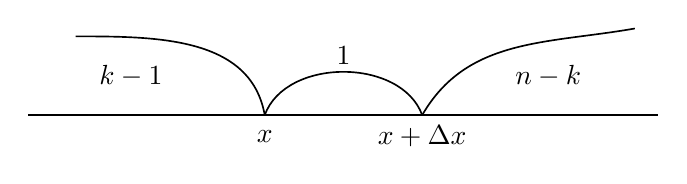
\begin{tikzpicture}[semithick]
        \draw(-4,0)--(4,0);\coordinate(a)at(-1,0);\node[below=2pt]at(a){$x$};
        \coordinate(b)at(1,0);\node[below]at(b){$x+\Delta x$};
        \draw[out=100,in=0](a)to(-3.4,1);
        \draw[out=70,in=110](a)to(b);
        \node at(0,0.75){$1$};\node at(-2.7,0.5){$k-1$};
        \draw[out=60,in=190](b)to(3.7,1.1);
        \node at(2.6,0.5){$n-k$};
    \end{tikzpicture}
    \caption{$X_{(k)}$取值的示意图}
\end{figure}

\begin{proposition}
    若$X_1,X_2,\dotsc,X_n$独立同分布,则次序统计量$(x_{(i)},x_{(j)})(i<j)$的联合分布密度函数为:
    \[ f_{ij}(y,z)=\frac{n!}{(i-1)!(j-i-1)!(n-j)!}[F(y)]^{i-1}[F(z)-F(y)]^{j-i-1} [1-F(z)]^{n-j}f(y)f(z),\ y \le z \]
\end{proposition}
\begin{proof}
    对正$\Delta y,\Delta z$以及$y<z$,事件``$x_{(i)}\in(y,y+\Delta y],x_{(j)}\in(z,z+\Delta z] $''可以表示为``容量为$n$的样本$x_1,\dotsc,x_n$中有$i-1$个观测值小于等于$y$,一个落入区间$(y,y+\Delta y],j-i-1$个落入区间$(y+\Delta y,z] $,一个落入区间$(z,z+\Delta z] $,而余下$n-j$个大于$z+\Delta z$''(见图~\ref{fig:5.3.6} ).
    \begin{figure}[!ht]
        \centering
        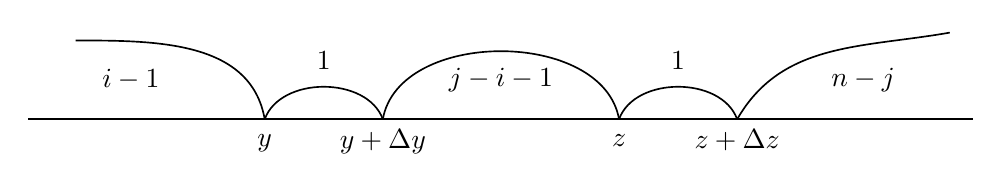
\begin{tikzpicture}[semithick]
            \draw(-6,0)--(6,0);
            \coordinate(a) at(-3,0);\coordinate(b)at(-1.5,0);
            \coordinate(c)at(1.5,0);\coordinate(d)at(3,0);
            \node[below=2pt]at(a){$y$};\node[below]at(b){$y+\Delta y$};
            \node[below=2pt]at(c){$z$};\node[below]at(d){$z+\Delta z$};
            \draw[out=100,in=0](a)to(-5.4,1);
            \draw[out=70,in=110](a)to(b);\draw[out=70,in=110](c)to(d);
            \node at(-2.25,0.75){$1$};\node at(-4.7,0.5){$i-1$};
            \draw[out=60,in=190](d)to(5.7,1.1);
            \node at(4.6,0.5){$n-j$};\node at(0,0.5){$j-i-1$};
            \draw[out=80,in=100](b)to(c);
            \node at(2.25,0.75){$1$};
        \end{tikzpicture}
        \caption{$x_{(i)}$与$x_{(j)}$取值的示意图}\label{fig:5.3.6}
    \end{figure}
\end{proof}

\begin{example}
    若$X_1,X_2,\dotsc,X_n$独立同分布, 求$R=X_{(n)}-X_{(1)}$的分布
\end{example}
\begin{solution}
    \[ f_{X_{(1)}X_{(n)}}(s,t)=n(n-1)f(s)f(t)[F(t)-F(s)]^{n-2}\mathbb{I}(s\le t) \]
    \[ f_R(r)=\mathbb{I}(r>0)\int_{-\infty}^{\infty}f_{X_{(1)}X_{(n)}}(s,s+r)ds \]
\end{solution}

\begin{problemset}[错题记录]
    \item (茆2.6.5)设随机变量$X$服从$(-\pi/2,\pi/2)$上的均匀分布,求随机变量$Y=\cos X$的密度函数$p_Y(y)$.
    \item (茆3.1.1)100件产品中有50件一等品,30件二等品,20件三等品。从中抽取 5 件,以$X$、$Y$分别表示取出的 5 件中一等品、二等品的件数,在以下情况下求$(X,Y)$的联合分布列:(1)不放回抽取;(2)有放回抽取。
    \item (茆3.1.7)设二维随机变量$(X,Y)$的联合密度函数为
    \[ p(x, y)=\begin{cases}
            4 x y, & 0<x<1,0<y<1,  \\
            0,     & \text{其他} .
        \end{cases}	\]
    试求
    \begin{enumerate}[(1)]
        \item$P(X<Y)$;
        \item$(X,Y)$的联合分布函数.
    \end{enumerate}
    \item (茆3.1.12)设二维随机变量$(X,Y)$的联合密度函数为
    \[
        p(x,y)=\begin{cases}
            x^2+\frac{xy}{3}, & 0<x<1,0<y<2;  \\
            0,                & \text{其他} .
        \end{cases}
    \]
    求$P(X+Y)\geq 1$.
    \item (茆3.1.16)设二维随机变量$(X,Y)$的联合分布函数为$F(x,y)$,试用$F(x,y)$表示$P(X=a,Y>b)$
    \item (茆3.3.4)设随机变量$X,Y$独立且都服从几何分布,即$P(X=k)=(1-p)^{k-1}p,k=1,2,\ldots$求随机变量$Z=\max\{X,Y\}$的分布列.
    \item (茆3.3.14)设二维随机变量$(X,Y)$在矩形
    \[ G=\{(x,y)|0 \le x \le 2,0 \le y \le 1\} \]
    上服从均匀分布, 试求边长分别为$X$和$Y$的矩形面积$Z$的密度函数.
    \item (茆3.3.17)设$X,Y \overset{\text{i.i.d.}}{\sim} N(0,1)$,试证明:$U=X^2+Y^2$与$V=\frac{X}{Y}$相互独立。
\end{problemset}
